\chapter{Android Application Development}

\section{Choice of Platform}

We chose Android as the target platform because it remains the most popular mobile operating system globally, holding approximately 70\% of the market share as of 2025. While cross-platform solutions like React Native, Flutter, or Xamarin offer the advantage of developing for multiple platforms simultaneously, they often come with trade-offs, such as reduced access to native device features, performance overhead, or difficulties integrating specific hardware functionalities. Given our application's requirements for real-time image processing and machine learning integration, native Android development provided the necessary performance and access to device-specific capabilities.

\section{Application Architecture}

The Android application was developed using Kotlin and structured as follows:

\begin{itemize}
\item \textbf{UI Layer}: Contains theming elements such as color schemes, typography, and theme configurations using Jetpack Compose (a modern toolkit for building native UI in Android~\cite{jetpack_compose}). This simplifies the management of visual consistency throughout the app.
\item \textbf{Domain Layer}: Includes core logic and data structures, such as the Classification data class, the IClassifier interface, and image processing helpers. Additionally, it contains the ImageAnalyzer, which manages the analysis of camera frames for classification.
\item \textbf{Data Layer}: Handles the integration and execution of the TensorFlow Lite model through the TfLiteClassifier class. This includes loading the model, preparing images for inference, and providing classification results to the domain layer.
\item \textbf{Root Layer}: Comprises main components directly tied to the application's functionality, such as screens (Home, Gallery, ExhibitDetailScreen, PhotoScanner) and navigation between these screens.
\end{itemize}

The architecture follows a modular approach, enabling clear separation of concerns between presentation, domain logic, and data processing. The UI layer is implemented entirely with Jetpack Compose, which allows for declarative and reactive UI construction. The domain layer acts as the application's logic core. By defining interfaces such as \texttt{IClassifier}, the code allows for easy swapping or extension of classification backends in the future. The data layer encapsulates the integration with machine learning models, abstracting away the details of TensorFlow Lite inference. Navigation and screen composition are handled in the root layer.

The diagram~\ref{fig:architecture} illustrates these layers and their interactions, showing data flow and relationships.

\begin{figure}[h]
    \centering
    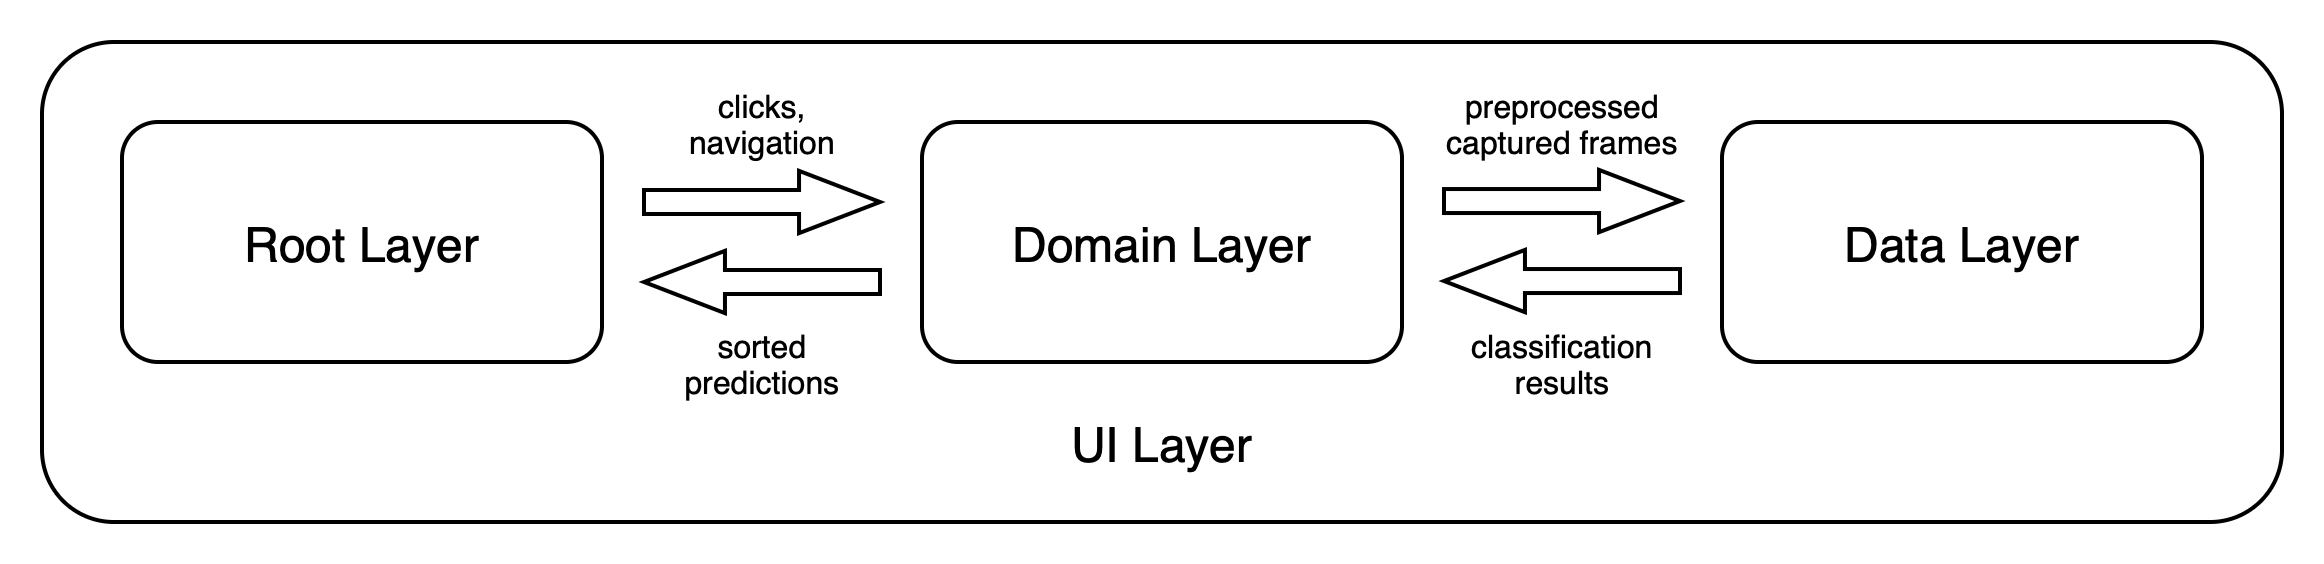
\includegraphics[width=\textwidth]{img/architecture-diagram.png}
    \caption{Application architecture diagram. The UI Layer handles theming, the Domain Layer contains core logic and data structures, the Data Layer integrates TensorFlow Lite, and the Root Layer manages screens and navigation.}\label{fig:architecture}
\end{figure}

\section{User Interface}

There are five main screens in the application:

\begin{itemize}
\item \textbf{Home Screen}: A page dedicated to the museum, with contacts and social media links.
\item \textbf{Gallery Screen}: A page displaying a grid of museum exhibits, allowing users to browse through available items and open detailed information about each exhibit.
\item \textbf{Exhibit Detail Screen}: A page providing information about an exhibit, such as title, author, and dates.
\item \textbf{Photo Scanner Screen}: Presents real-time recognition results directly overlaid on the live camera view.
\item \textbf{Classification Result Screen}: Displays the classification results, showing the top recognized exhibit and up to four alternatives for user selection ordered by confidence level. This is particularly useful for misclassified or uncertain results, allowing users to find the correct exhibit.
\end{itemize}

In Figures~\ref{fig:app_screens_1} and~\ref{fig:app_screens_2}, you can see the application's user interface, showcasing the main screens and some additional details, such as permission requests and debug mode. Additionally, a short video demonstrating the usage of the application can be viewed at the following link: 

\begin{center}
\url{https://www.youtube.com/shorts/RytfYy3VI8E}
\end{center}

\begin{figure}[h]
    \centering

    \begin{subfigure}[b]{0.3\textwidth}
        \centering
        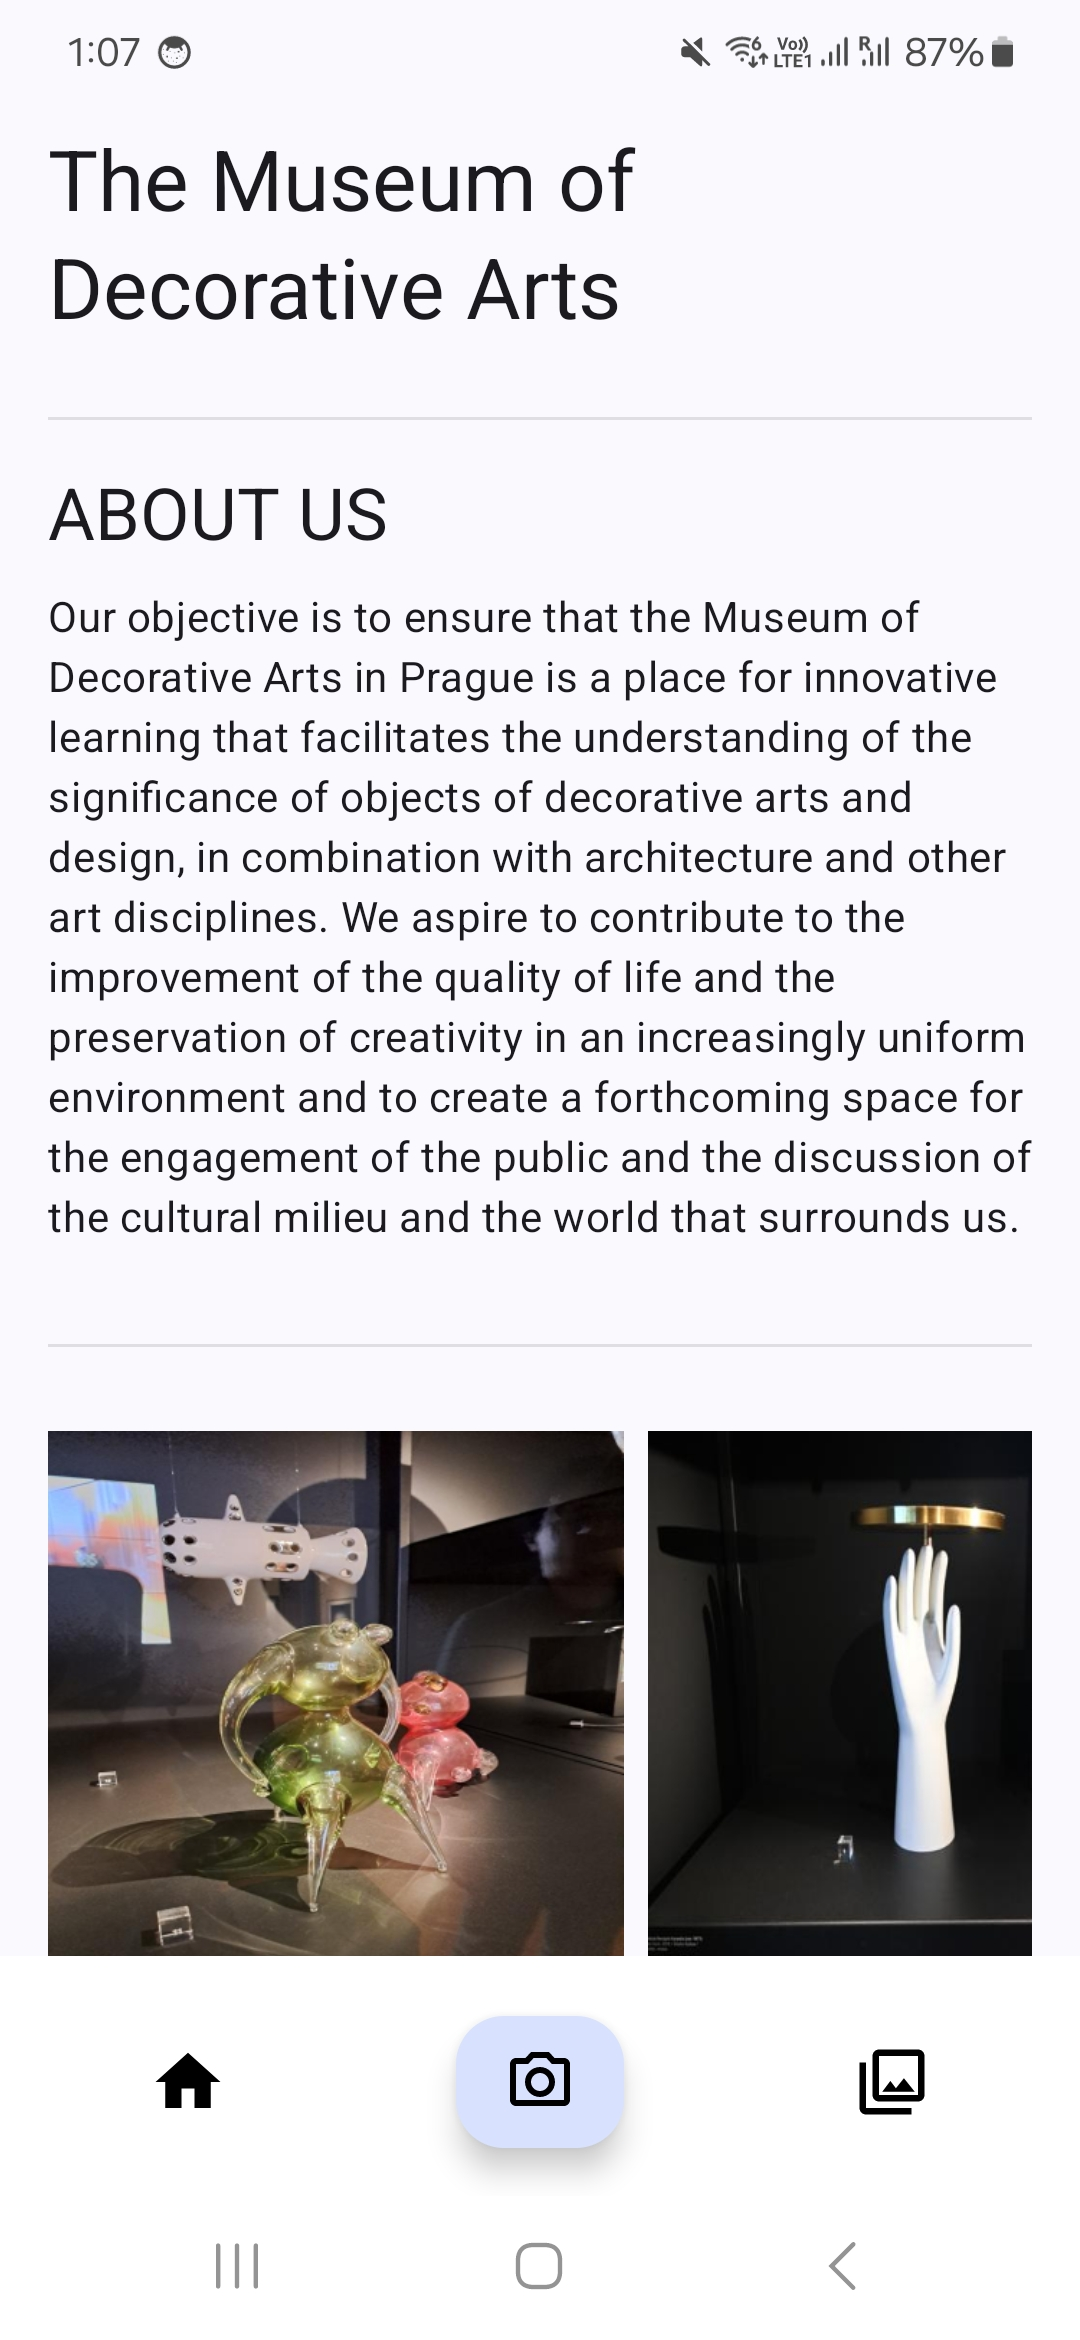
\includegraphics[width=\textwidth]{img/home-screen-1.jpg}
        \caption{Home Screen (1/2).}
    \end{subfigure}
    \hfill
    \begin{subfigure}[b]{0.3\textwidth}
        \centering
        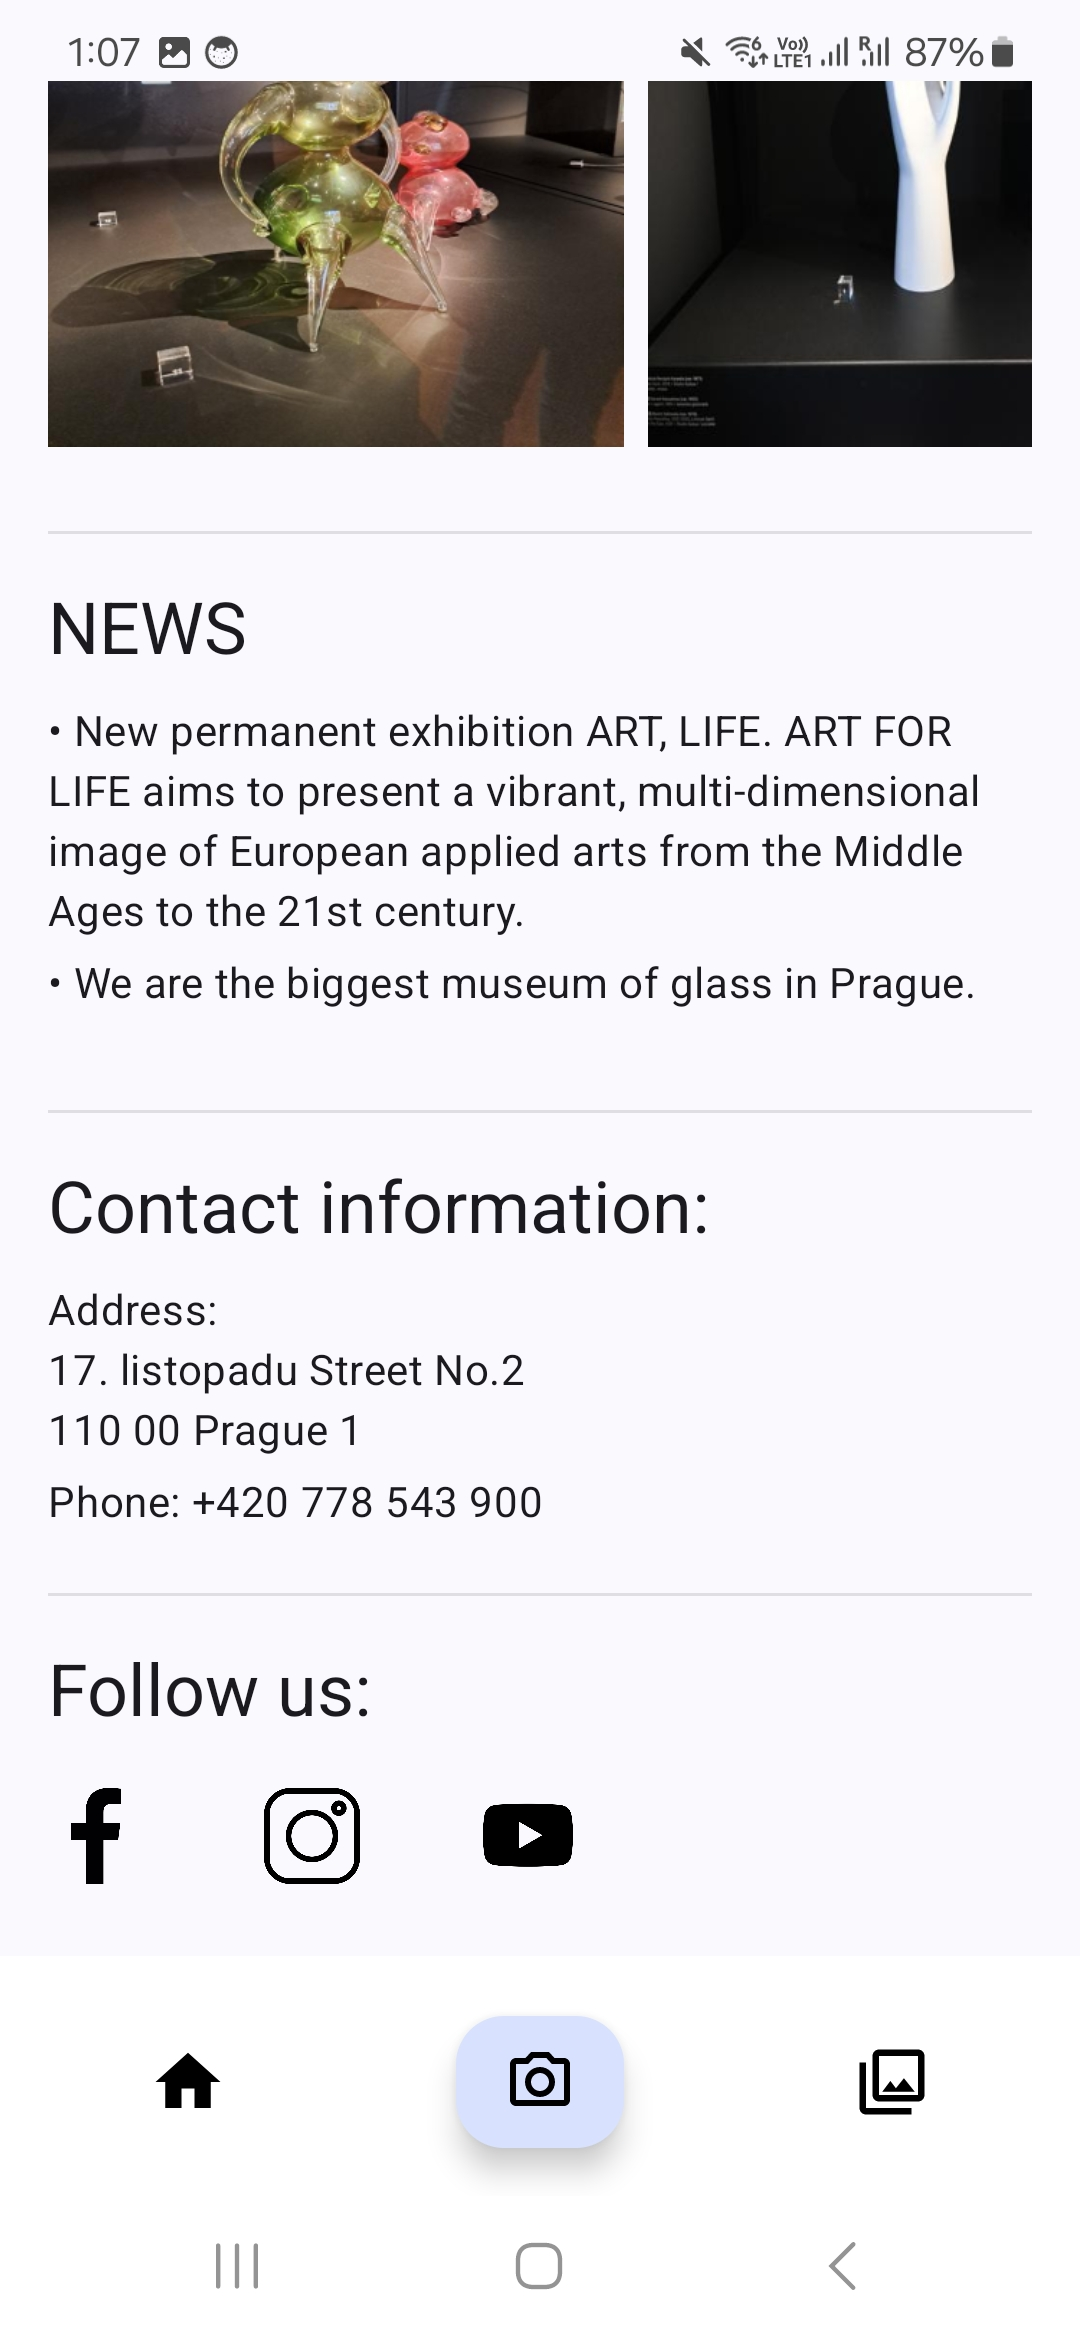
\includegraphics[width=\textwidth]{img/home-screen-2.jpg}
        \caption{Home Screen (2/2).}
    \end{subfigure}

    \vspace{1em}

    \begin{subfigure}[b]{0.3\textwidth}
        \centering
        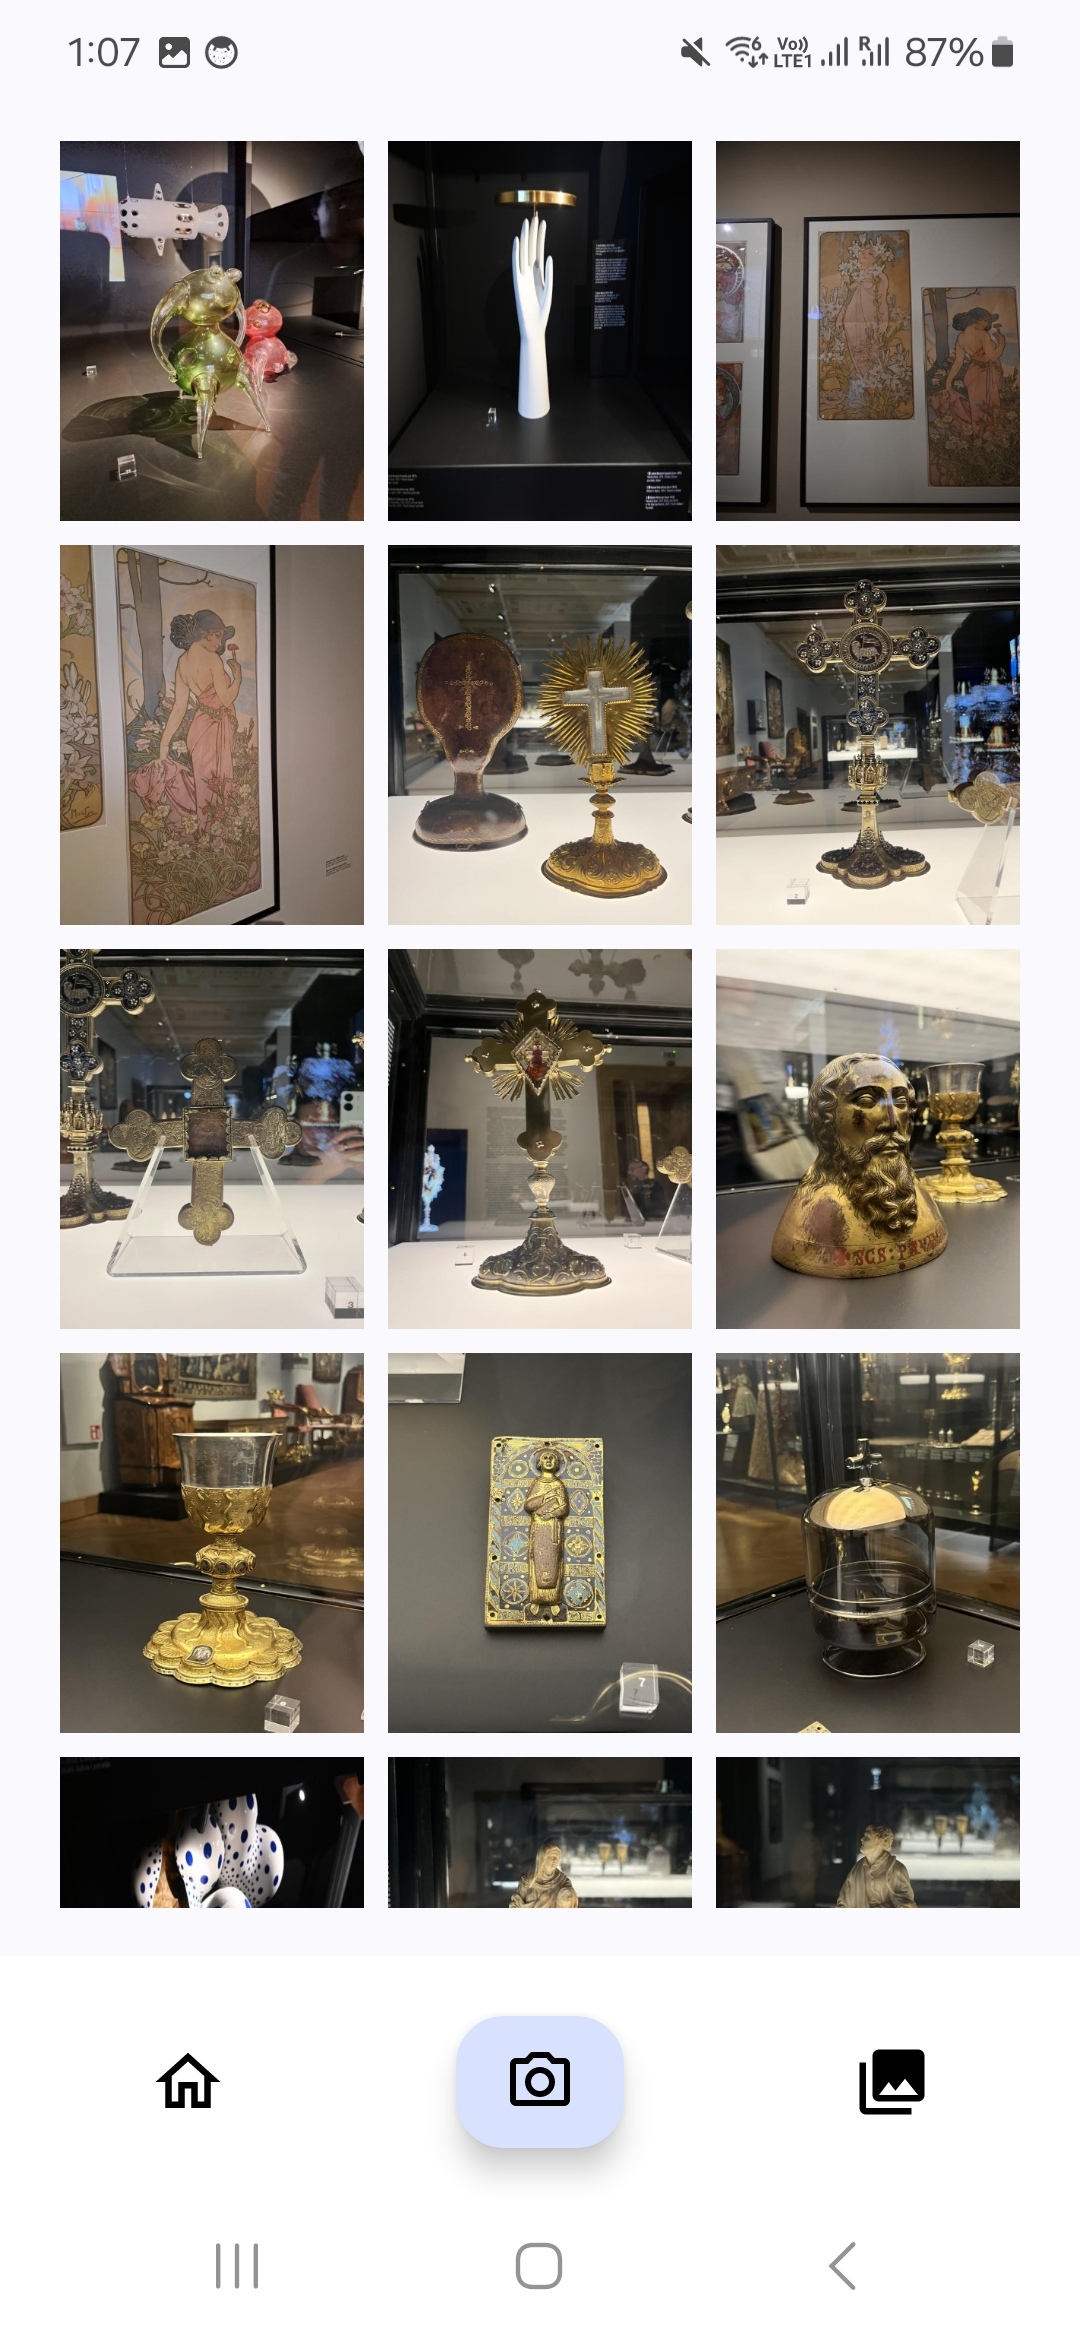
\includegraphics[width=\textwidth]{img/gallery-screen.jpg}
        \caption{Gallery Screen.}
    \end{subfigure}
    \hfill
    \begin{subfigure}[b]{0.3\textwidth}
        \centering
        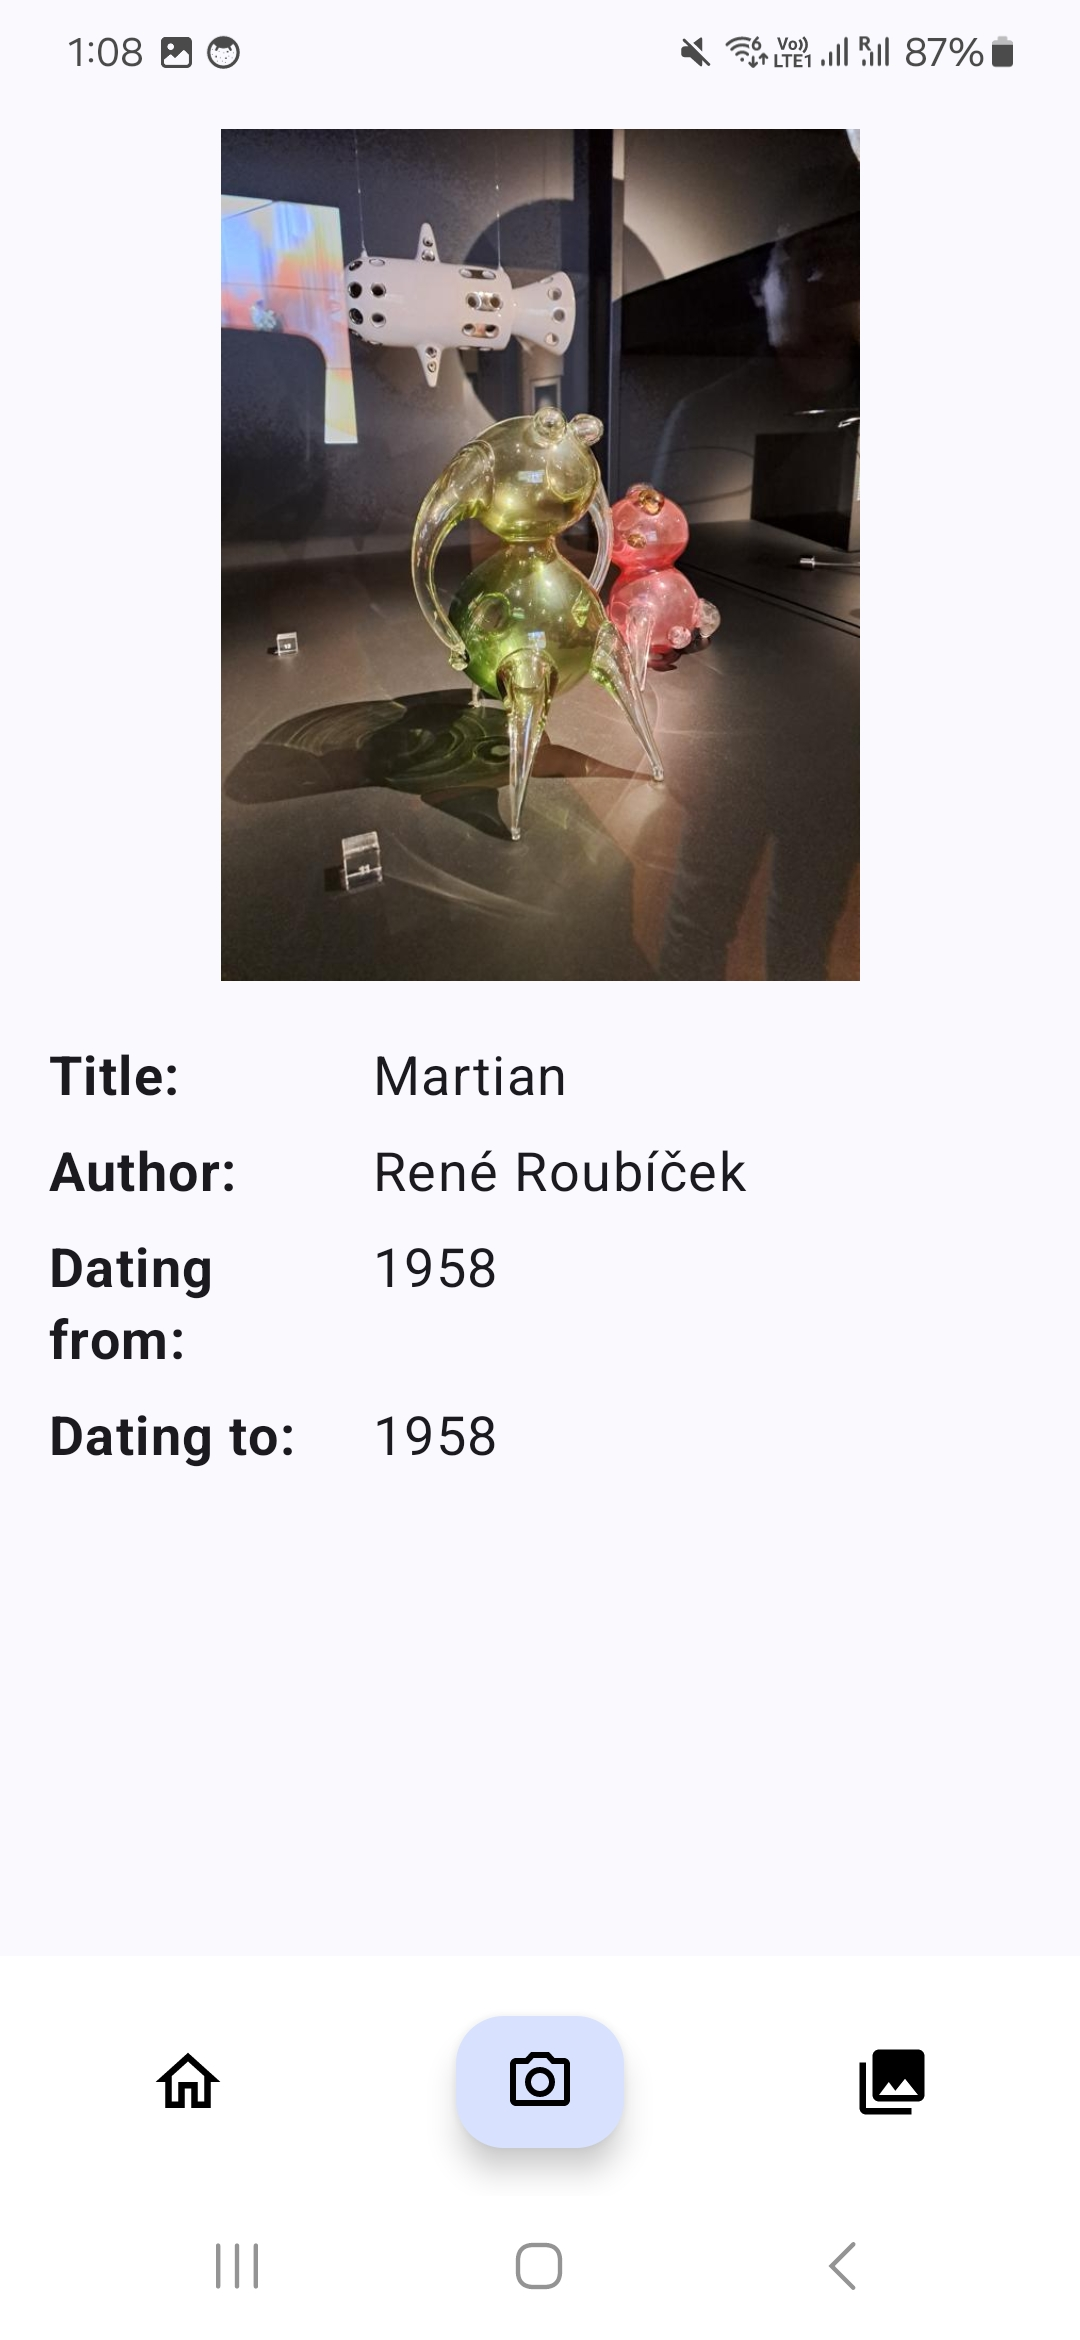
\includegraphics[width=\textwidth]{img/exhibit-screen.jpg}
        \caption{Exhibit Detail Screen.}
    \end{subfigure}

    \caption{Screens of the application. The Home Screen provides museum information, the Gallery Screen displays exhibits, and the Exhibit Detail Screen shows detailed information about a selected exhibit.}\label{fig:app_screens_1}
\end{figure}

\begin{figure}[h]
    \centering

    \begin{subfigure}[b]{0.3\textwidth}
        \centering
        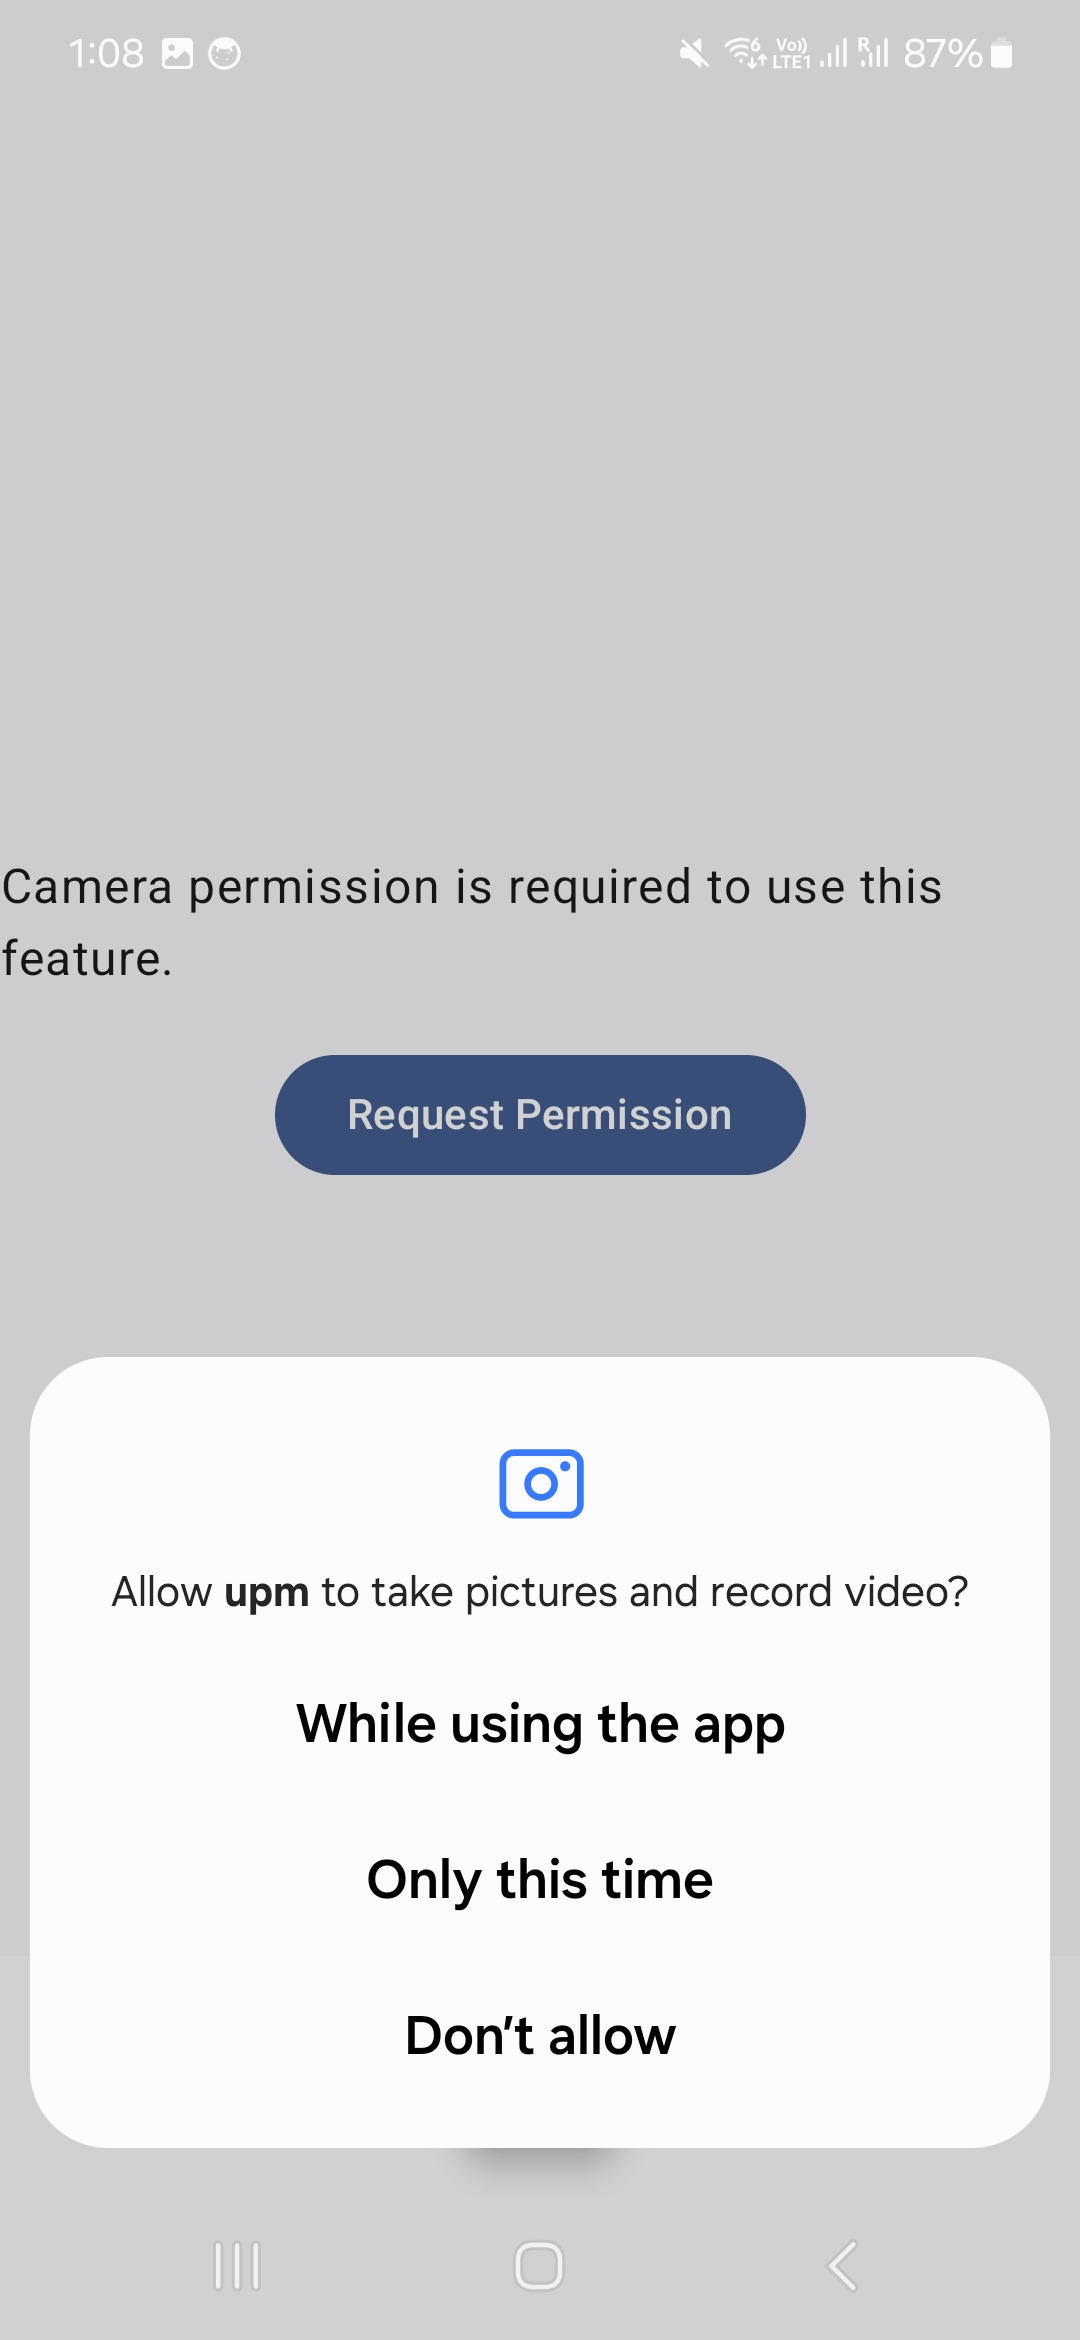
\includegraphics[width=\textwidth]{img/permissions-screen.jpg}
        \caption{Permissions.}
    \end{subfigure}
    \hfill
    \begin{subfigure}[b]{0.3\textwidth}
        \centering
        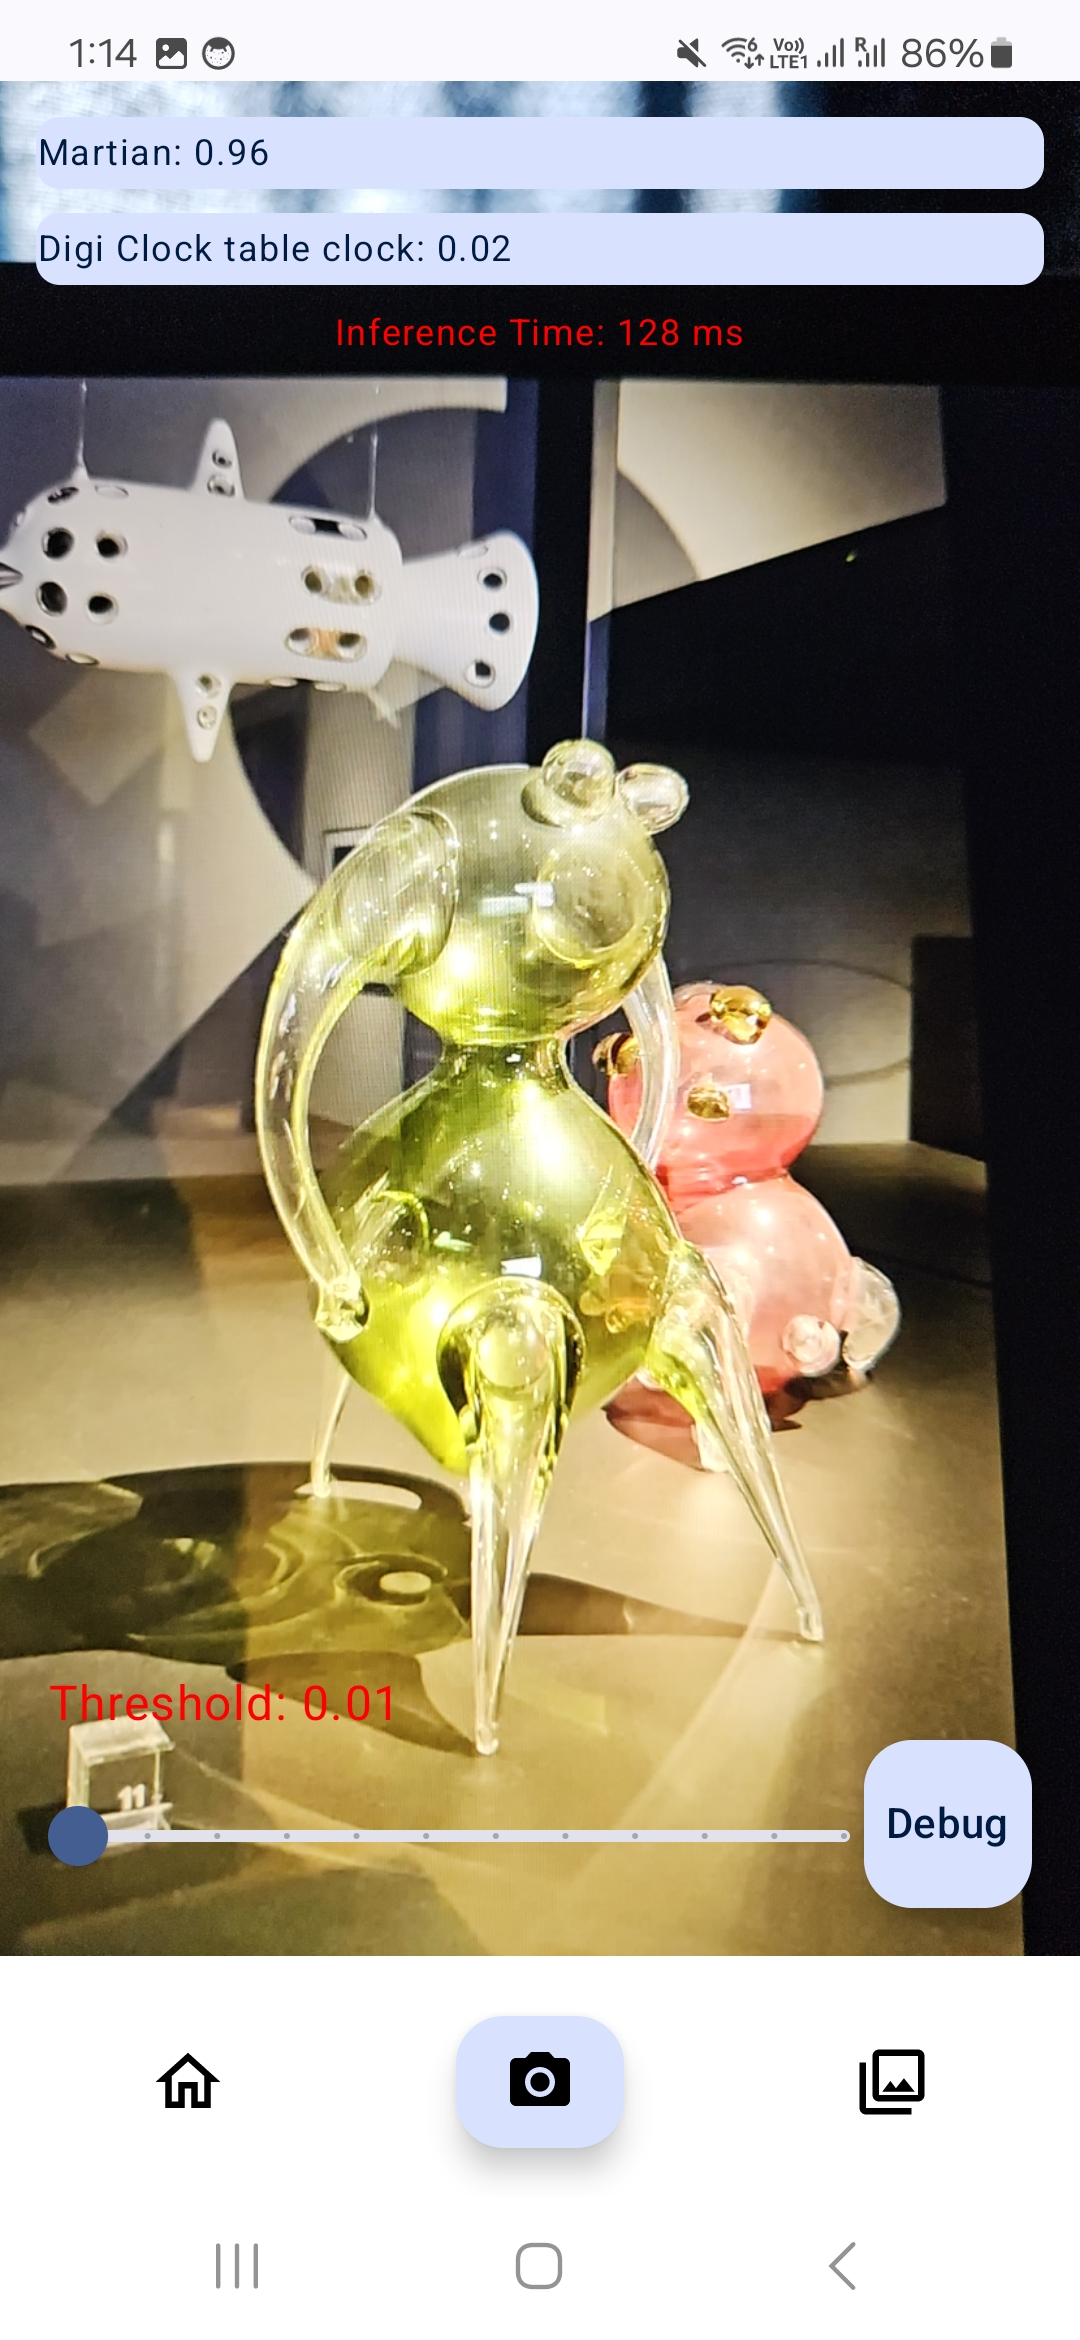
\includegraphics[width=\textwidth]{img/debug-mode.jpg}
        \caption{Debug Mode.}
    \end{subfigure}

    \vspace{1em}

    \begin{subfigure}[b]{0.3\textwidth}
        \centering
        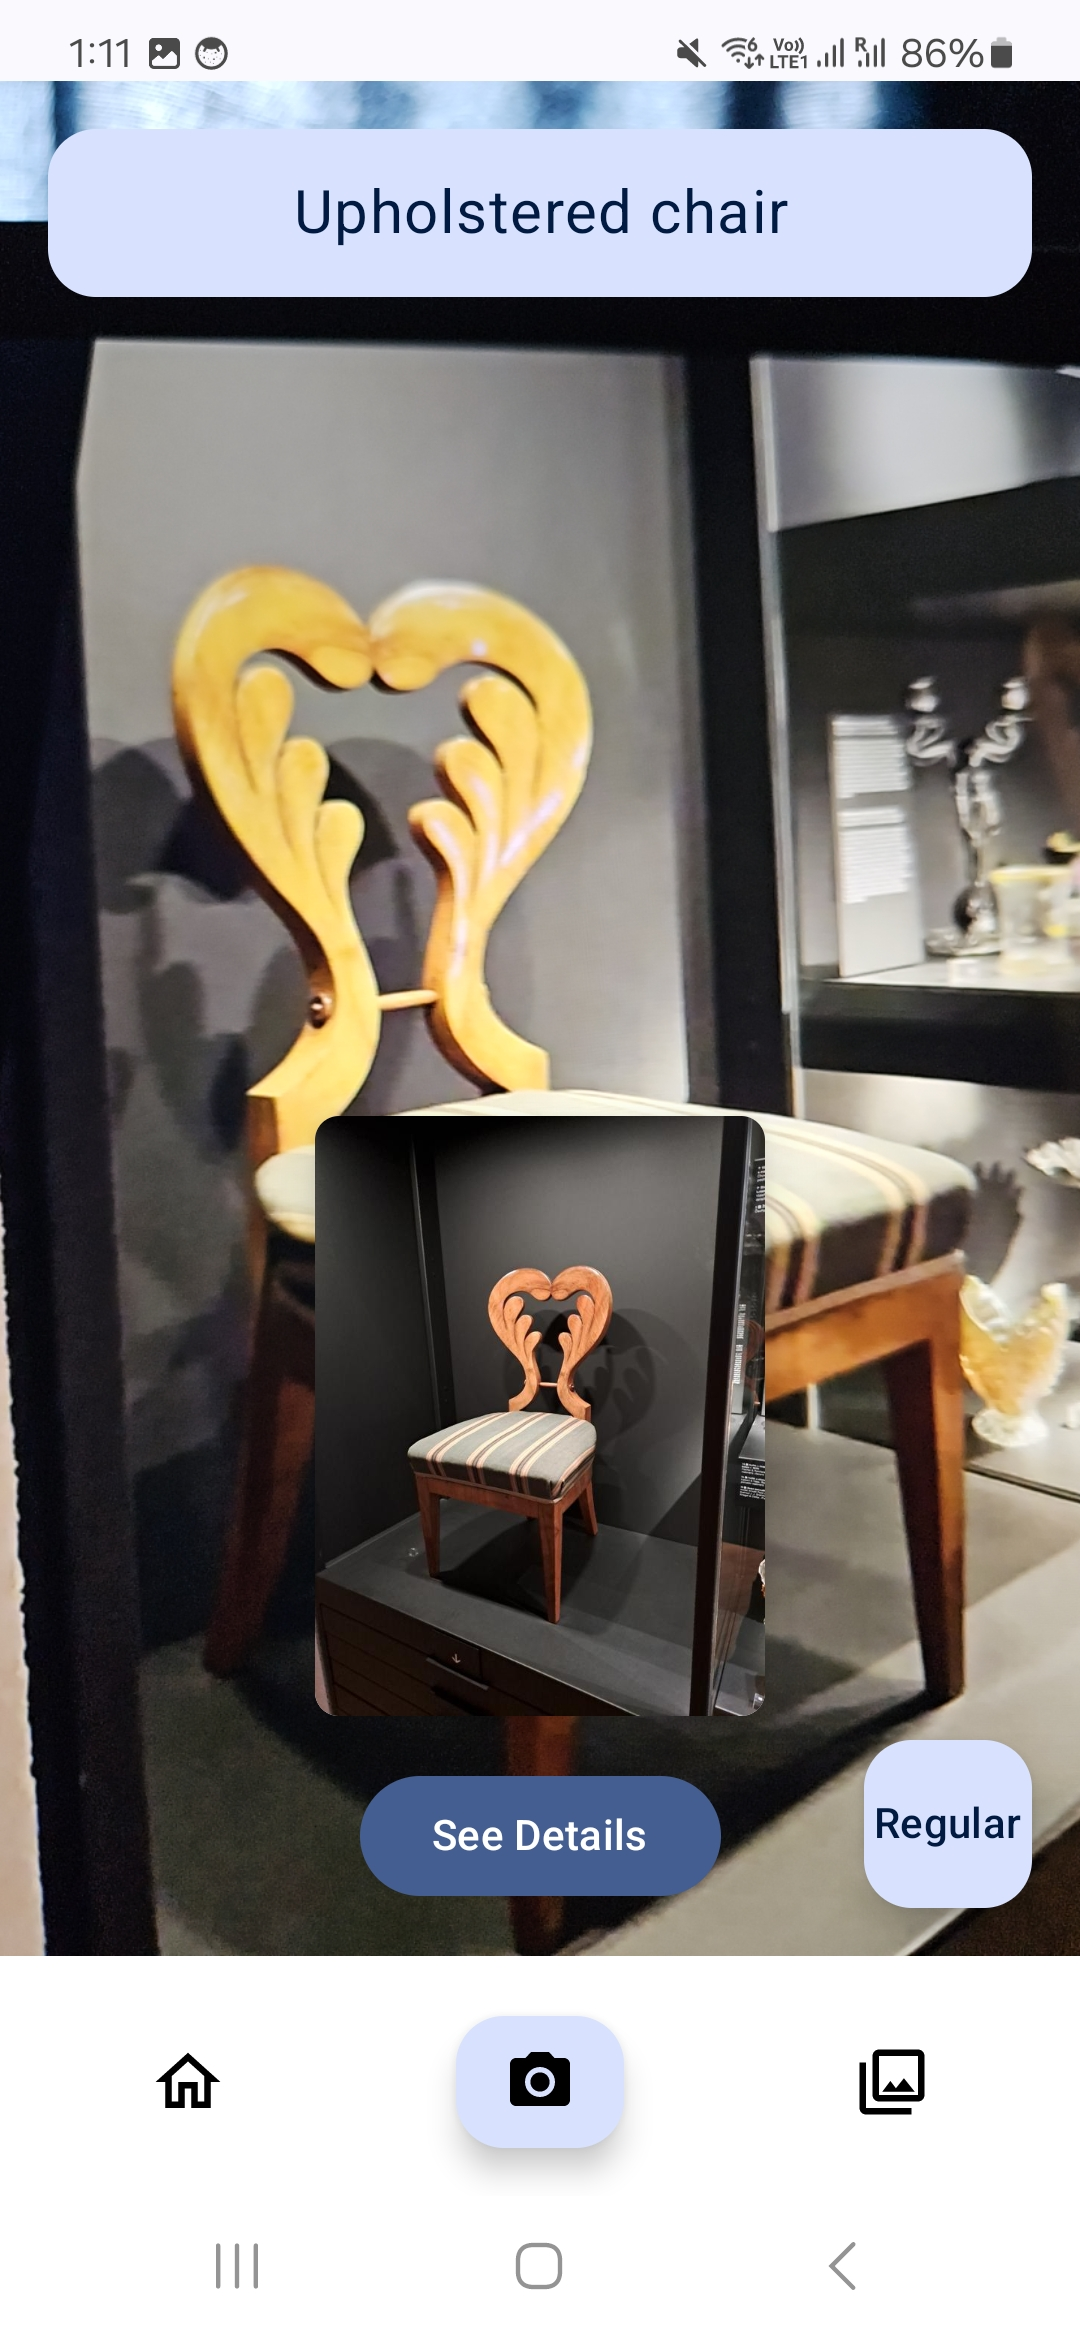
\includegraphics[width=\textwidth]{img/classification-preview-screen.jpg}
        \caption{Photo Scanner Screen.}
    \end{subfigure}
    \hfill
    \begin{subfigure}[b]{0.3\textwidth}
        \centering
        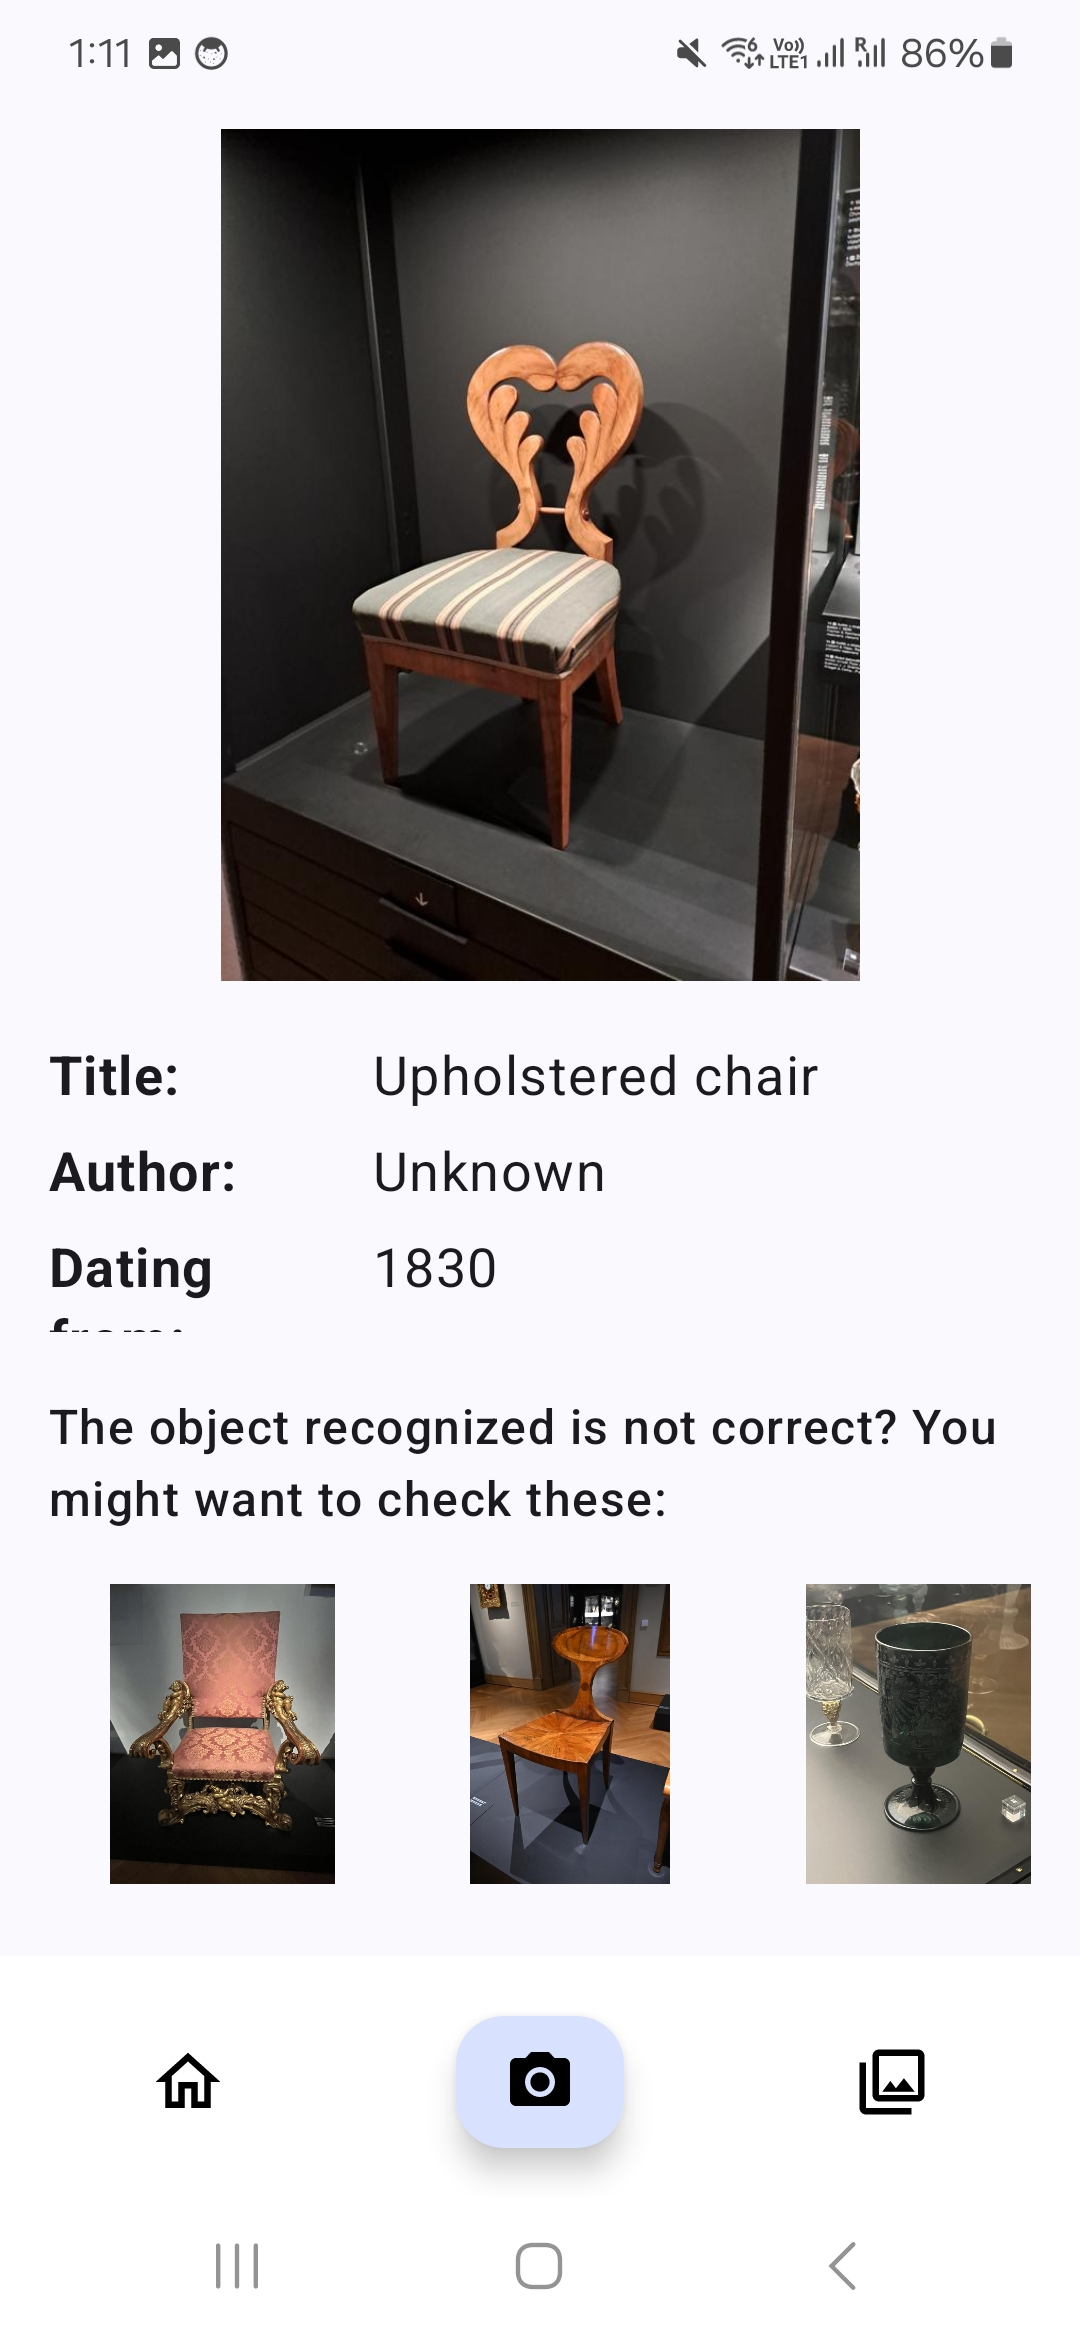
\includegraphics[width=\textwidth]{img/classification-screen.jpg}
        \caption{Classification Result Screen.}
    \end{subfigure}

    \caption{Screens of the application. The Permissions screen requests necessary permissions, the Debug Mode allows for real-time adjustments, the Photo Scanner Screen shows the live camera feed with recognition results, and the Classification Result Screen displays the top recognized exhibit and alternatives.}\label{fig:app_screens_2}
\end{figure}

\section{Real-Time Image Processing and TensorFlow Lite Integration}

To make our application recognize museum exhibits in real-time, we combined the capabilities of TensorFlow Lite (TFLite) with Android's CameraX library~\cite{camerax}. TensorFlow Lite allows machine learning models to run efficiently directly on mobile devices, while CameraX makes it straightforward to access and manage the device's camera hardware across various Android phones.

When the application starts, it loads the MobileNetV2 TFLite model we trained. This initial loading is done once.

Next, CameraX continuously captures frames from the camera. To avoid overwhelming the device, our application analyzes only every 30th frame captured by the camera. This balance provides timely recognition without putting too much strain on the phone's resources.

Each captured frame is initially in YUV format, a standard camera format optimized for speed and efficiency. However, our model requires standard Bitmap images, representing image data in the RGB color space. Therefore, each selected YUV frame is converted into a Bitmap.

After converting to a Bitmap, we preprocess the image further by resizing it to $224 \times 224$ pixels to match the input dimensions of the MobileNetV2 model. Additionally, each pixel's values are normalized, adjusting them from the original 0--255 range into a 0--1 range. This normalization is crucial for the model to interpret the pixel values correctly, as it was trained on images in this normalized format.

Once preprocessed, the Bitmap is sent to the TensorFlow Lite model, which performs the classification task. The model analyzes the image and returns a set of predictions, ranking them based on confidence levels. These results are then sent to the UI, where users can see the recognized exhibit and alternative suggestions to help with possible misclassifications.

By integrating CameraX for capturing frames and TensorFlow Lite for image recognition, we created an efficient, responsive application that provides museum visitors with immediate and reliable exhibit identification.

\section{Threshold Adjustment}

An important parameter in the classification process is the classification threshold, which determines the minimum confidence level required for a prediction to be considered valid. If the model's confidence in the top prediction is below this threshold, the application will not display any results, indicating uncertainty in the classification. 

To provide the user with some result and its alternatives in most cases, but not overload the user with likely irrelevant results, we set the threshold to 0.3.

\section{Debug Mode}

To get more insights into the model's behaviour in a real scenario (while testing the application in the museum), we implemented a debug mode. This mode can be activated by clicking a button on the camera preview screen. When enabled, it allows changing the model's threshold on the fly and displays all classification results with a confidence level above the threshold (alongside their confidence levels). This feature is particularly useful for deciding on the optimal threshold for the model, as it allows one to see the range of usual confidence levels for correct classifications. The debug mode also displays the time taken for each classification, which will help us evaluate the model's responsiveness.

\section{Final Pipeline}

The complete pipeline for the application's core functionality can be described step-by-step as follows:

\begin{enumerate}
\item \textbf{User Interaction and Navigation (UI and Root Layers)}:
\begin{itemize}
\item \textbf{Input}: User interactions (clicks, navigations).
\item \textbf{Output}: Navigation to appropriate screens (e.g., PhotoScanner).
\end{itemize}

\item \textbf{Input Acquisition (CameraX, Domain Layer)}:
\begin{itemize}
    \item \textbf{Input}: Real-time camera feed (YUV format).
    \item \textbf{Output}: Selected frames at defined intervals (every 30th frame).
\end{itemize}

\item \textbf{Image Preprocessing (Bitmap Conversion and Normalization, Domain Layer)}:
\begin{itemize}
    \item \textbf{Input}: YUV image frames.
    \item \textbf{Process}: Conversion from YUV to RGB Bitmap format, resizing to $224 \times 224$ pixels, and normalization of pixel values from 0--255 to 0--1 range.
    \item \textbf{Output}: Normalized Bitmap images ready for classification.
\end{itemize}

\item \textbf{TensorFlow Lite Model Inference (Data Layer)}:
\begin{itemize}
    \item \textbf{Input}: Preprocessed Bitmap images.
    \item \textbf{Process}: Inference performed using the preloaded MobileNetV2 TFLite model, configured with adjustable threshold parameters.
    \item \textbf{Output}: Classification results including the recognized exhibit labels, IDs, and confidence scores.
\end{itemize}

\item \textbf{Result Processing and Filtering (Domain Layer)}:
\begin{itemize}
    \item \textbf{Input}: Raw classification results.
    \item \textbf{Process}: Filtering based on confidence threshold (default 0.3), sorting results by confidence, and selection of top predictions.
    \item \textbf{Output}: Final set of results with one primary prediction and up to four alternative predictions.
\end{itemize}

\item \textbf{User Interface Presentation (UI Layer)}:
\begin{itemize}
    \item \textbf{Input}: Processed classification results.
    \item \textbf{Process}: Results are displayed in the UI overlaying the camera preview, highlighting the primary identified exhibit, with quick access to alternative suggestions.
    \item \textbf{Output}: Interactive display allowing the user to navigate to detailed exhibit information.
\end{itemize}

\item \textbf{Exhibit Information Display (Root and UI Layer)}:
\begin{itemize}
    \item \textbf{Input}: Exhibit ID from classification results.
    \item \textbf{Process}: Retrieval of detailed exhibit information from CSV data.
    \item \textbf{Output}: Detailed exhibit view including title, author, dating information, and related imagery.
\end{itemize}
\end{enumerate}

This comprehensive overview should provide a better understanding of the holistic behavior and integration of the various elements in the application.

\section{Conclusion}

In this chapter, we have described in detail the development of our Android application, focusing on the choice of platform, architecture, user interface design, and integration of real-time image processing with TensorFlow Lite. The application is designed in such a way as to ensure user-friendliness while efficiently using the device's resources to recognize exhibits in real time. The combination of CameraX and TensorFlow Lite allows you to effectively classify museum exhibits, increasing visitor engagement and interaction with the museum's offerings.